\subsection*{\textbf{\textit{RQ3: How well can we model the delivery delay of addressed issues?}}}

\begin{figure}
	\centering
	%\captionsetup{justification=centering}
	\subfloat[Eclipse]{
		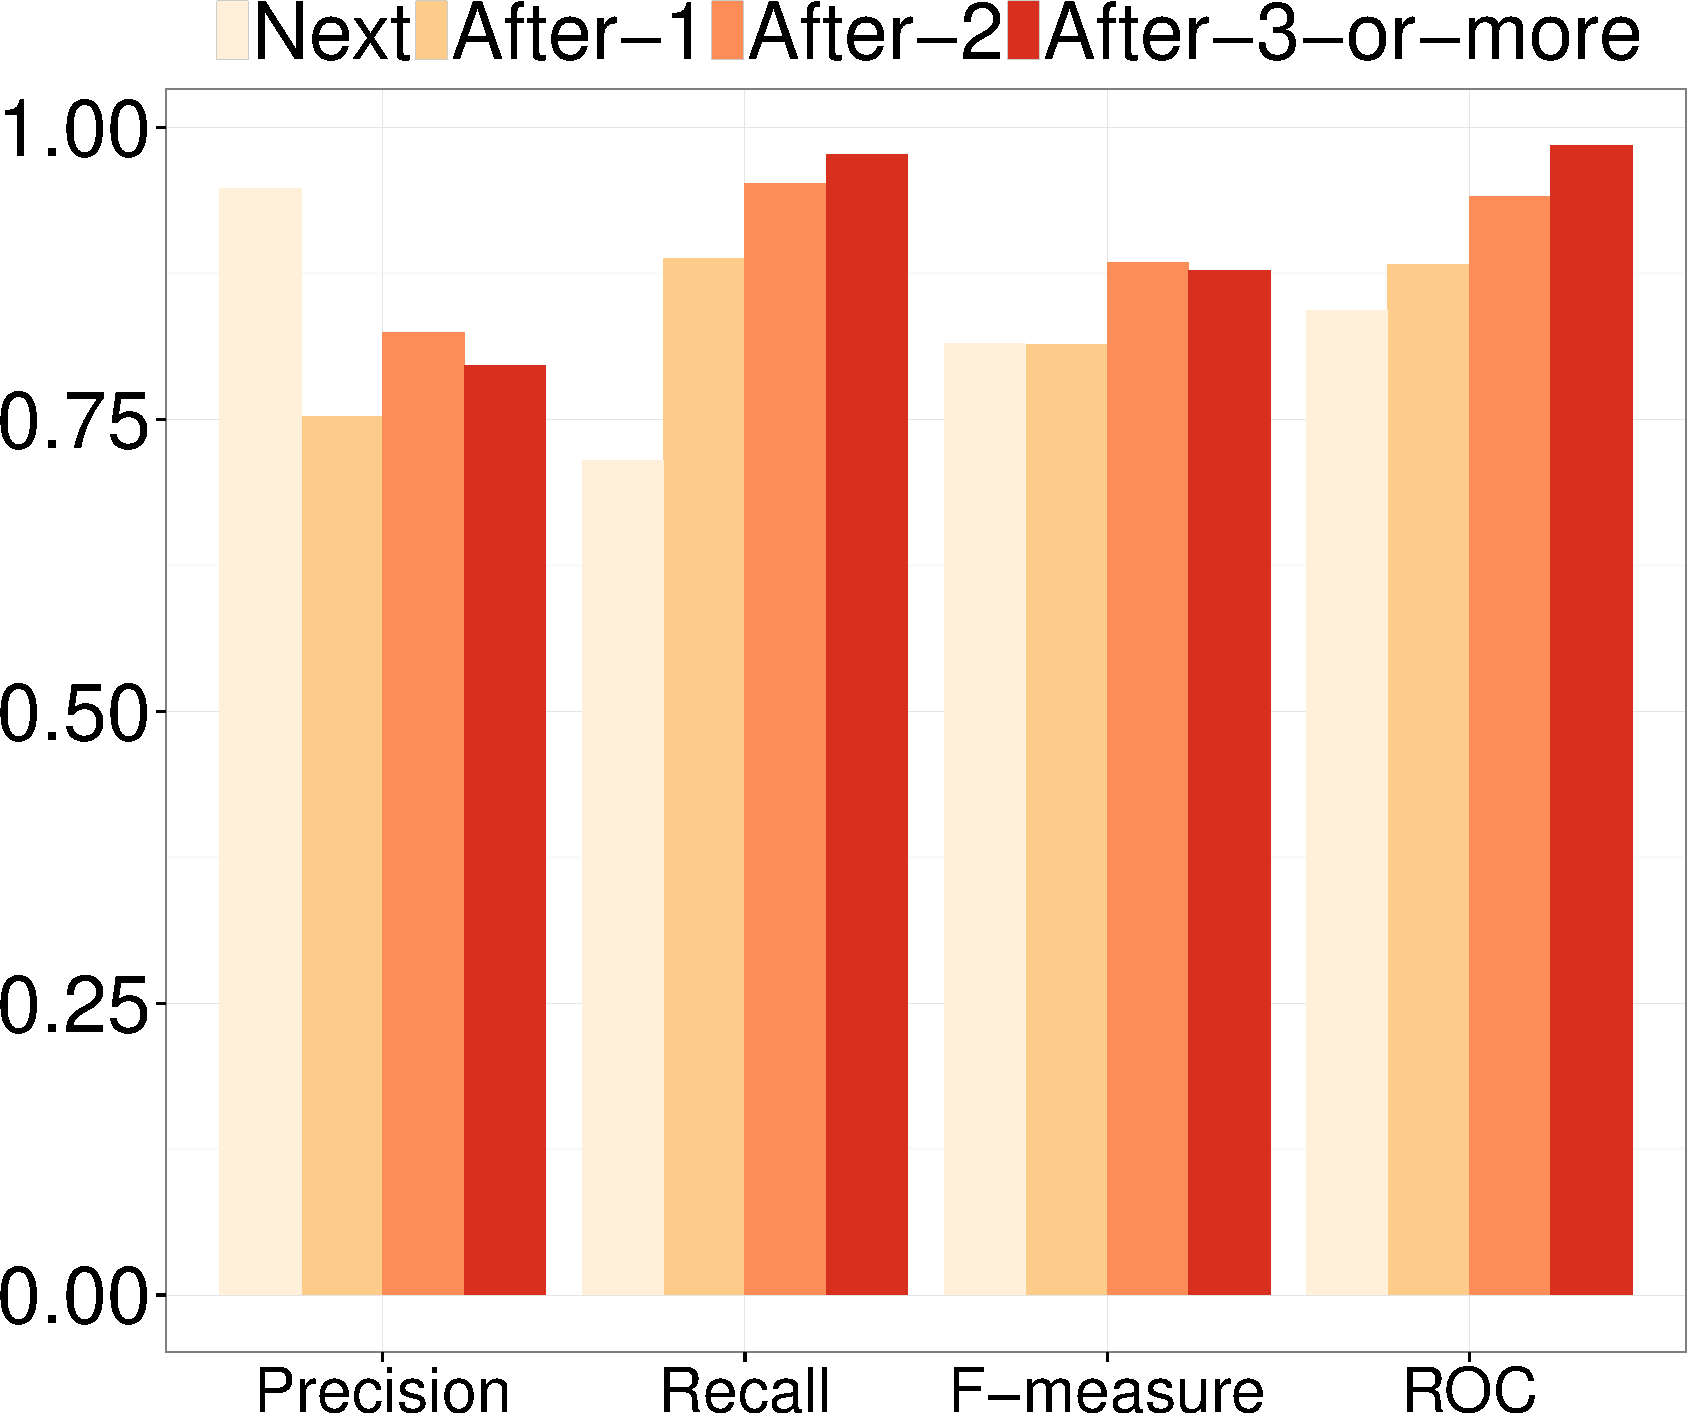
\includegraphics[width=0.50\textwidth,keepaspectratio] 
		{chapters/chapter4/figures/eclipse_loocv_evaluation.pdf}
		\label{ch4:fig:RFeclipse}
	}

	\subfloat[Firefox]{
		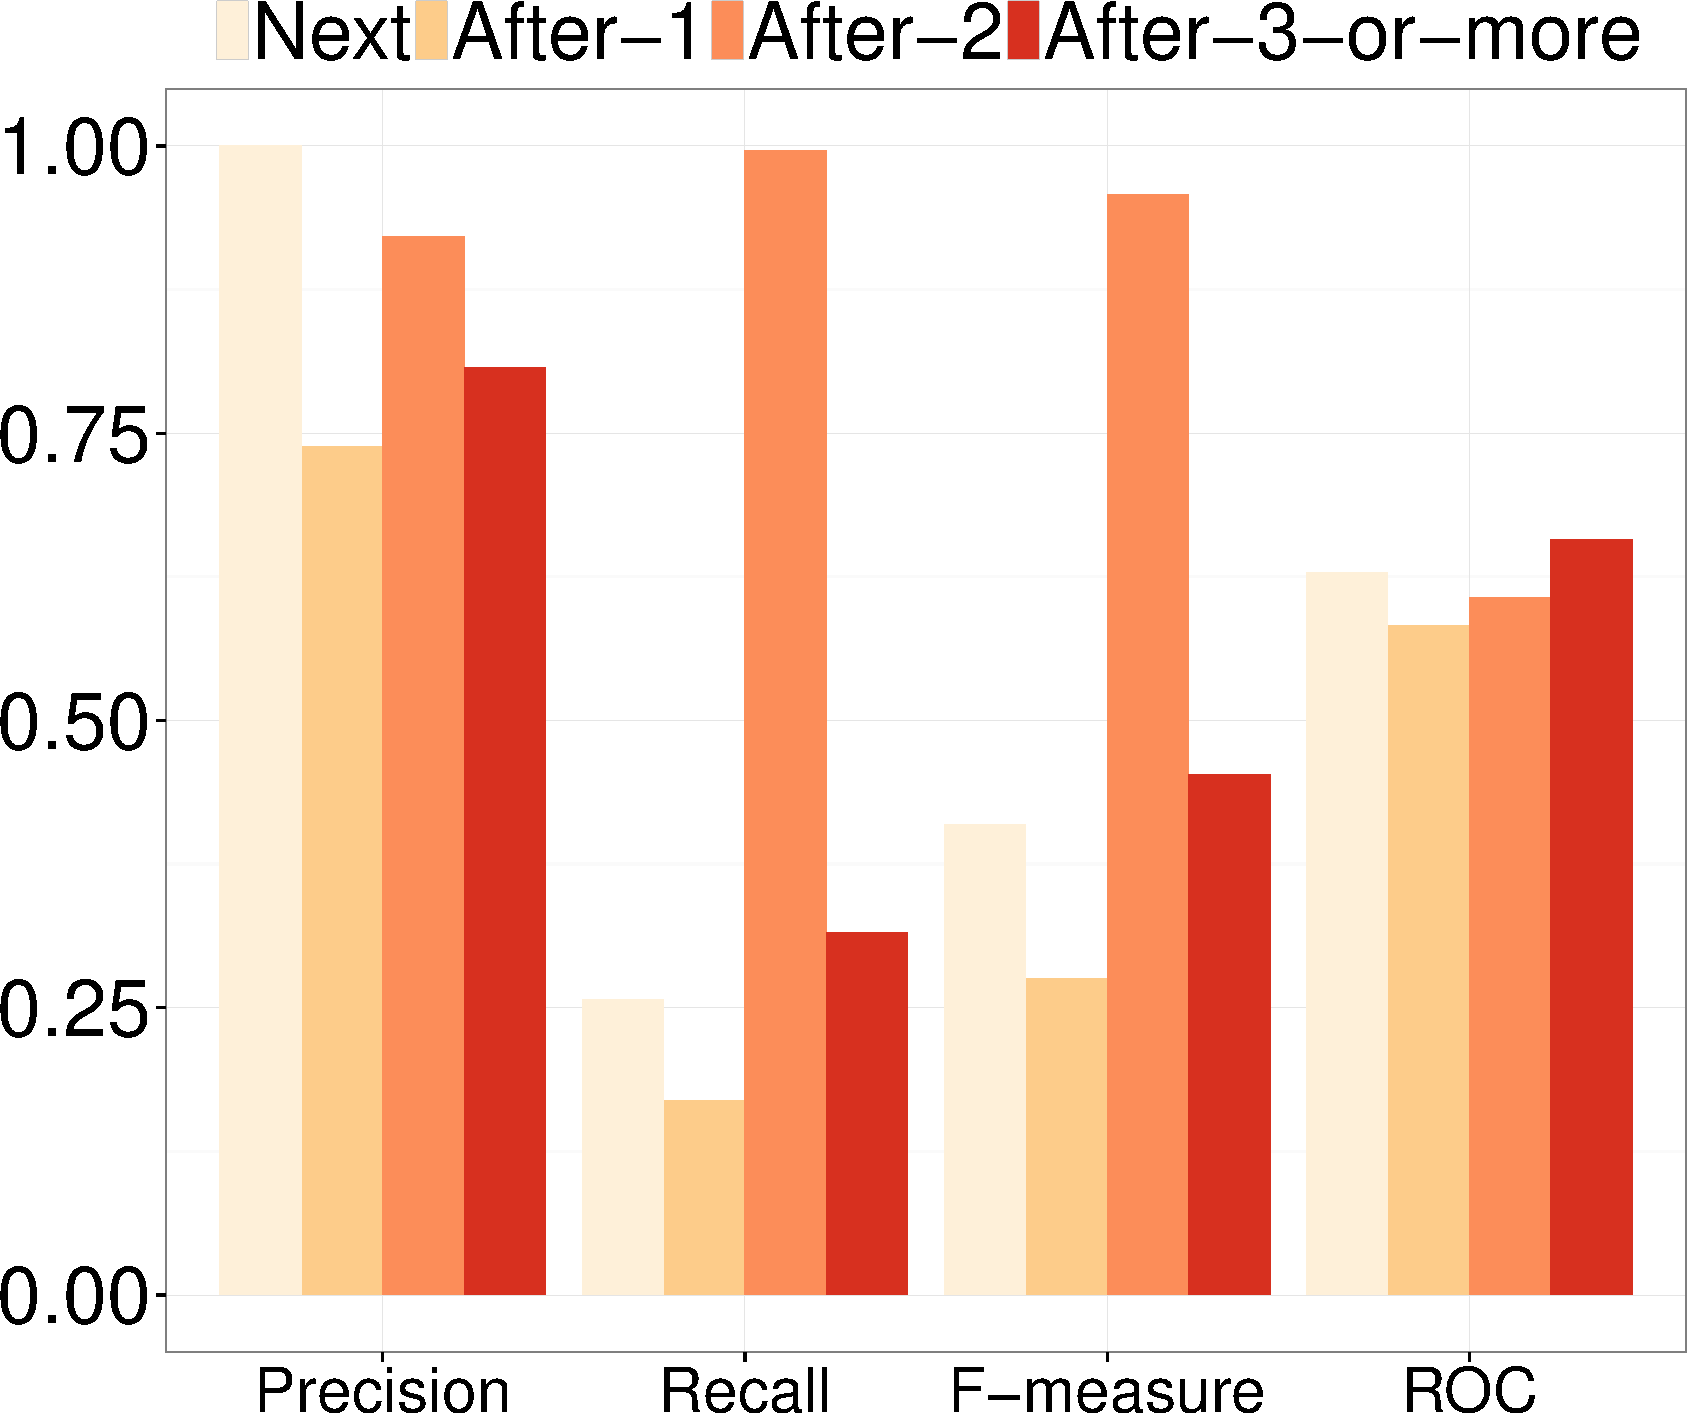
\includegraphics[width=0.50\textwidth,keepaspectratio]  
		{chapters/chapter4/figures/firefox_loocv_evaluation.pdf}
		\label{ch4:fig:RFfirefox}
	}

	\subfloat[ArgoUML]{
		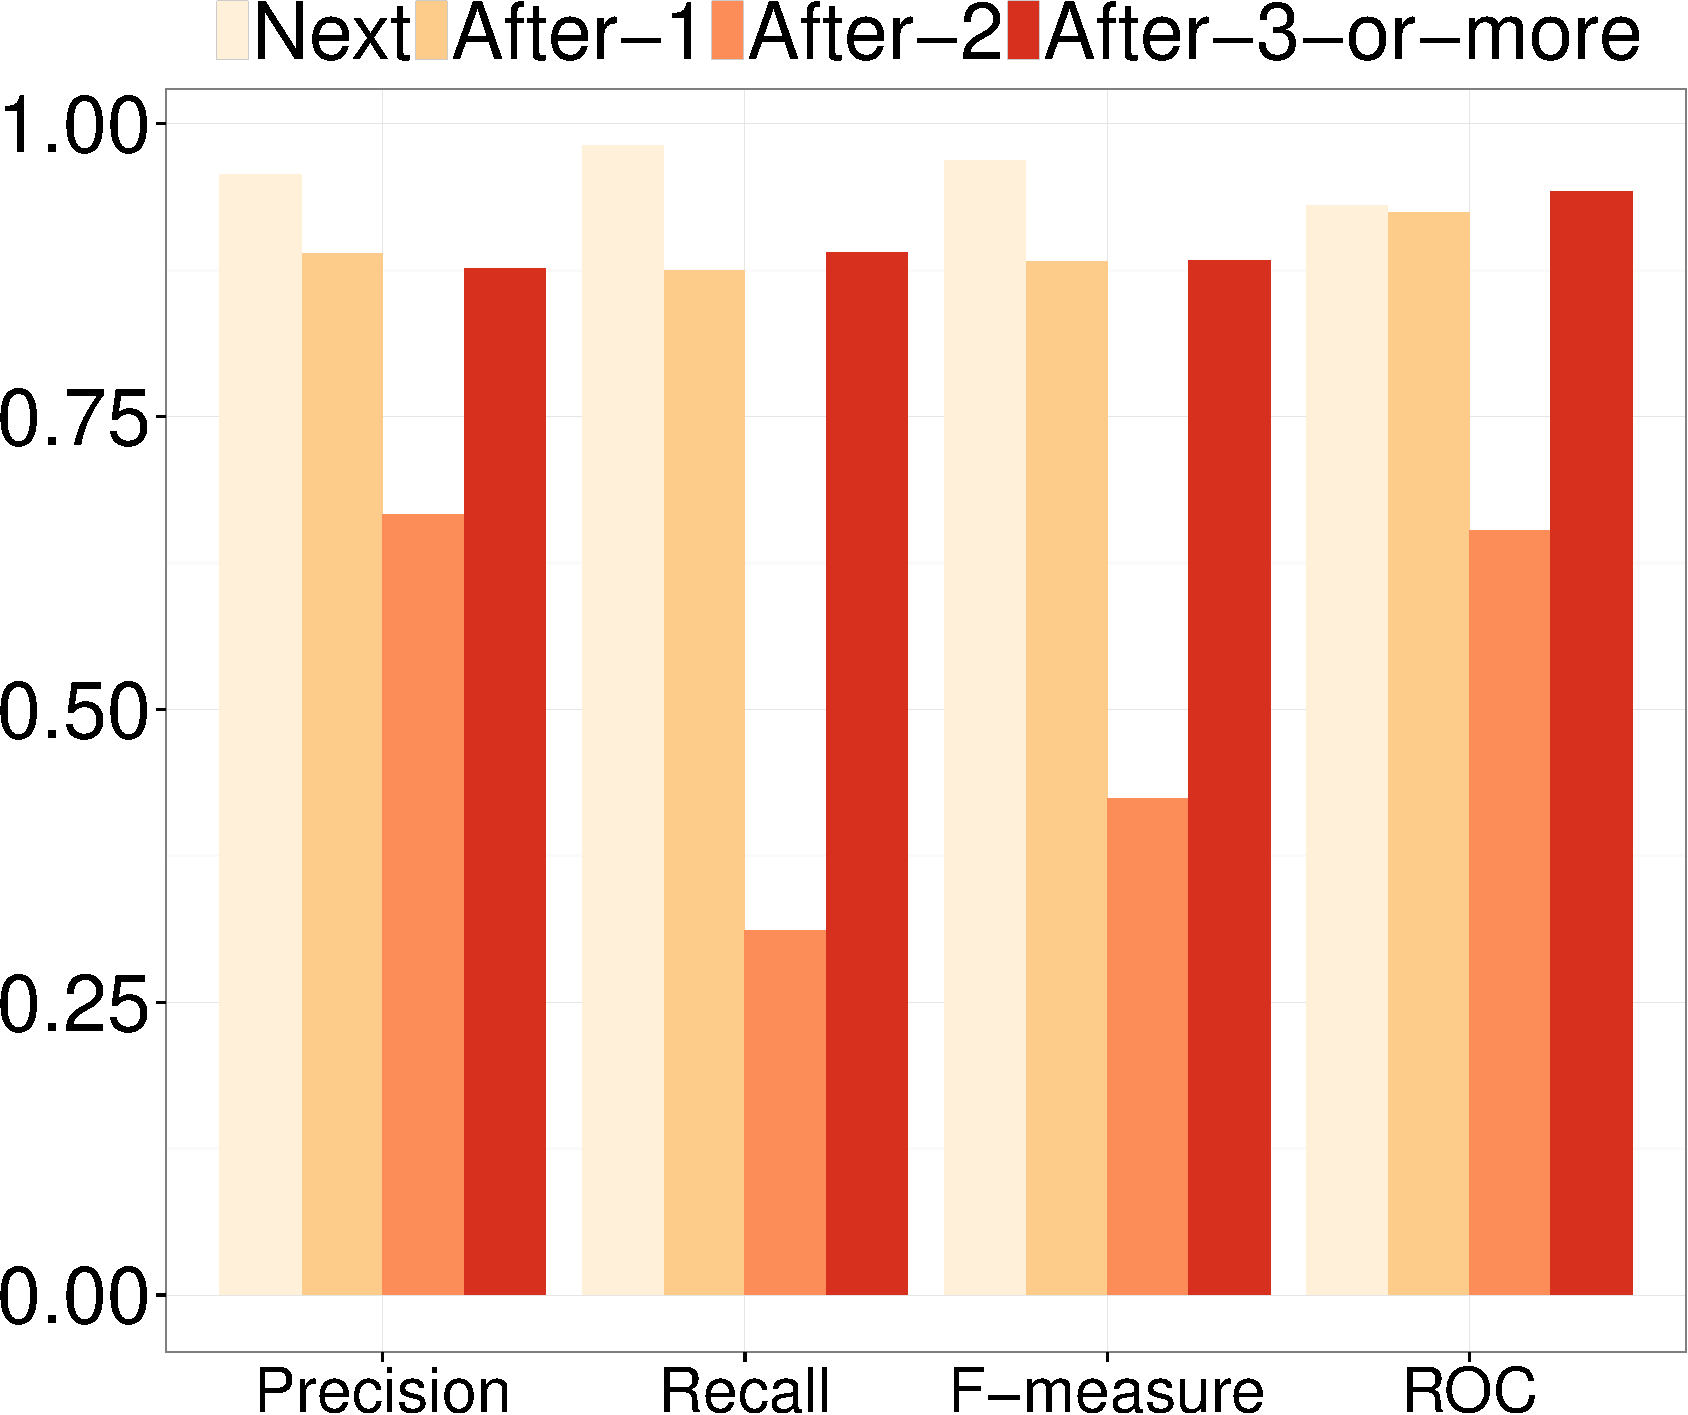
\includegraphics[width=0.50\textwidth,keepaspectratio] 
		{chapters/chapter4/figures/argouml_loocv_evaluation.pdf}
		\label{ch4:fig:RFargo}
	}
	\caption{\textbf{Performance of random forest models.} We show the
	values of Precision, Recall, F-measure, and AUC that are
computed using the LOOCV technique.}
	\label{ch4:fig:RFclassificationResult}
\end{figure}

\begin{table}
	\footnotesize
	\centering
	\caption{The precision, recall, F-measure, and AUC values that are
	obtained for the Eclipse, Firefox, and ArgoUML projects. 
	\label{ch4:tbl:evaluation_metrics}
	}
	\begin{tabular}{lcccc}
		\hline
		\multicolumn{5}{c}{\textbf{Eclipse}}\tabularnewline
		\hline 
		\textbf{Bucket} & \textbf{Precision} & \textbf{Recall} &
		\textbf{F-measure} & \textbf{AUC}\tabularnewline
		\hline 
		Next & 0.95  & 0.71  & 0.81 & 0.84 \tabularnewline
		\hline 
		After-1 & 0.75 & 0.89 & 0.81 & 0.88\tabularnewline
		\hline 
		After-2 & 0.82 & 0.95 & 0.88 & 0.94\tabularnewline
		\hline 
		After-3-or-more & 0.80 & 0.98 & 0.88 & 0.98\tabularnewline
		\hline 
		\hline
		\multicolumn{5}{c}{\textbf{Firefox}}\tabularnewline
		\hline 
		\textbf{Bucket} & \textbf{Precision} & \textbf{Recall} &
		\textbf{F-measure} & \textbf{AUC}\tabularnewline
		\hline 
		Next & 0.99  & 0.26  & 0.41 & 0.63 \tabularnewline
		\hline 
		After-1 & 0.74 & 0.17 & 0.28 & 0.58\tabularnewline
		\hline 
		After-2 & 0.92 & 0.99 & 0.96 & 0.61\tabularnewline
		\hline 
		After-3-or-more & 0.81 & 0.32 & 0.45 & 0.66\tabularnewline
		\hline 
		\hline
		\multicolumn{5}{c}{\textbf{ArgoUML}}\tabularnewline
		\hline 
		\textbf{Bucket} & \textbf{Precision} & \textbf{Recall} &
		\textbf{F-measure} & \textbf{AUC}\tabularnewline
		\hline 
		Next & 0.96  & 0.98  & 0.97 & 0.93 \tabularnewline
		\hline 
		After-1 & 0.89 & 0.87 & 0.88 & 0.92\tabularnewline
		\hline 
		After-2 & 0.67 & 0.31 & 0.42 & 0.65\tabularnewline
		\hline 
		After-3-or-more & 0.88 & 0.89 & 0.88 & 0.94\tabularnewline
		\hline 
	\end{tabular}
\end{table}

\subsubsection*{\textit{\textbf{RQ3: Results for delivery delay in terms of
releases}}}

\noindent\textit{\textbf{Our explanatory models obtain a median precision of 0.81 to
0.88 and a median recall of 0.29 to 0.92.}}
\hyperref[ch4:fig:RFclassificationResult]{Figure}~\ref{ch4:fig:RFclassificationResult}
shows the precision, recall, F-measure, and AUC of our explanatory models.  The
bar charts show the values that we observe for each bucket. The values of
precision, recall, F-measure, and AUC are also shown in
\hyperref[ch4:tbl:evaluation_metrics]{Table}~\ref{ch4:tbl:evaluation_metrics}. 

The best precision/recall values that we obtain for the Eclipse, Firefox, and
ArgoUML projects are related to the \textit{after-2} (F-measure of 0.88),
\textit{after-2} (F-measure of 0.96), and \textit{next} (F-measure of 0.97),
respectively. However, for buckets with low number of instances,
precision/recall values decrease considerably. For instance, the F-measures that
are obtained by our models for the Firefox project are considerably low for the
\textit{next}, \textit{after-1}, and \textit{after-3-or-more} buckets (0.41,
0.28 and 0.45, respectively).

Moreover, our models obtain median AUCs between 0.62 to 0.96, which indicate
that our model estimations are better than random guessing (AUC of 0.5).
Summarizing the results, our models obtain a median precision of 0.81-0.88
(median) and a median recall of 0.29-0.92. Our models provide a sound starting
point for studying the release into which an addressed issue will be integrated.\\

\noindent\textit{\textbf{Our models obtain better F-measure values than
Zero-R.}} We compared our models to Zero-R models as a baseline. For all test
instances, Zero-R selects the bucket that contains the majority of the instances.
Hence, the recall for the bucket containing the majority of instances is 1.0. We
compared the F-measure of our models to the F-measure of Zero-R models. We
choose to compare to the F-measure values because precision and recall are very
skewed for Zero-R. 

For the Firefox project, Zero-R obtains an F-measure of 0.95 for the
\textit{after-2} bucket, whereas our model obtains an F-measure of 0.96 for the
same bucket. For the Eclipse project, Zero-R always selects \textit{next} and
obtains a F-measure of 0.58, while our model obtains an F-measure of 0.81.
Finally, for the ArgoUML project, Zero-R always selects \textit{next} with an
F-measure of 0.84, whereas our model obtains an F-measure of 0.97. These results
show that our models yield better F-measure values than na\"{i}ve techniques
like Zero-R or random guessing (AUC = 0.5) in the majority of cases.  

\conclusionbox{We are able to accurately model how many releases an addressed issue
is likely to be prevented from integration. Our models outperform na\"{i}ve
techniques, such as Zero-R and random guessing, obtaining AUC values of 0.62 to
0.96.}

\begin{table}
	\centering
	\footnotesize
	\caption{\textbf{Regression results of model fit.} Our explanatory
		models obtain $R^2$ values between 0.39 to 0.65 and MAE values between
	7.8 to 66 days.}
	\label{ch4:tbl:regression_results}
	\def\arraystretch{1.5}
	\begin{tabular}{lrrr}
		\hline 
		\centering{\textbf{Metric/Project}} &
		\centering{\textbf{Eclipse}} & \centering{\textbf{Firefox}} &
		\centering{\textbf{ArgoUML}} \tabularnewline
		\hline 
		$R^2$ & 0.48  & 0.39 & 0.65 \tabularnewline
		\hline 
		MAE (days) & 61 & 7.8  & 66 \tabularnewline
		\hline 
		Release cycle duration (median in days) & 112 & 42 & 180 \tabularnewline
		\hline
		Error ratio $(\frac{MAE}{cycle})$ & 0.54  & 0.18  & 0.37 \tabularnewline
		\hline 
		Optimism & 0.0267 & 0.0162 & 0.0035 \tabularnewline
		\hline 
	\end{tabular}
\end{table}

\subsubsection*{\textit{\textbf{RQ3: Results for delivery delay in terms of days}}}

\noindent\textbf{\textit{Our explanatory models obtain $R^2$ values of 0.39-0.65
and MAE values between 7.8 to 67 days.}} Our models obtain fair $R^2$ values to
model the variability of delivery delay in days in the studied projects.
\hyperref[ch4:tbl:regression_results]{Table}~\ref{ch4:tbl:regression_results} shows the
$R^2$ and MAE values that are obtained by each of our regression models. The
$R^2$ values for the Eclipse, Firefox, and ArgoUML projects are of 0.39, 0.48,
and 0.65, respectively. 
Additionally, our regression models can provide fair
estimations of delivery delay in days, specially for the Firefox project. For
instance, the median interval in days between releases of the Firefox project is
42 days
(see~\hyperref[ch4:fig:releaseIntervals]{Figure}~\ref{ch4:fig:releaseIntervals}), while
the MAE value for the Firefox project is 7.8 days, which equates to an error
ratio of 18\% (see
\hyperref[ch4:tbl:regression_results]{Table}~\ref{ch4:tbl:regression_results}).\\

\noindent\textbf{\textit{Our explanatory models obtain a good stability with bootstrap
calculated optimism between 0.0035 to 0.0267 of the $R^2$ values.}} We also
observe that our regression models are stable.
\hyperref[ch4:tbl:regression_results]{Table}~\ref{ch4:tbl:regression_results} shows the
\textit{bootstrap-calculated} optimism of the $R^2$ values of our models. The
optimism for the Eclipse, Firefox and ArgoUML projects are 0.0267, 0.0162, and 0.0035,
respectively. Such results indicate that our explanatory models are unlikely to
be overfitted to our data and that our models are stable enough for us to perform the
statistical inferences that follow. 

\conclusionbox{We are able to accurately estimate the delivery delay in terms
of number of days. Our models obtain fair $R^2$ values of 0.39 to 0.65. Our
exploratory models are quite stable with a maximum optimism of 0.0267.}

